
%(BEGIN_QUESTION)
% Copyright 2007, Tony R. Kuphaldt, released under the Creative Commons Attribution License (v 1.0)
% This means you may do almost anything with this work of mine, so long as you give me proper credit

When an acid substance is added to water, some of the acid molecules dissociate into positive hydrogen ions (H$^{+}$) and negative ions (the type of negative ions depending on what type of acid it is).  This increases the molarity of hydrogen ions (the number of moles of H$^{+}$ ions per liter of solution).  The addition of hydrogen ions to the solution also decreases the molarity of hydroxyl ions (the number of moles of OH$^{-}$ ions per liter of solution) because some of the water's OH$^{-}$ ions combine with the acid's H$^{+}$ ions to form deionized water molecules (H$_{2}$O).

\vskip 10pt

If an alkaline substance (otherwise known as a {\it caustic}, or a {\it base}) is added to water, some of the alkaline molecules dissociate into negative hydroxyl ions (OH$^{-}$) and positive ions (the type of positive ions depending on what type of alkaline it is).  This increases the molarity of OH$^{-}$ ions in the solution, as well as decreases the molarity of hydrogen ions (again, because some of the caustic's OH$^{-}$ ions combine with the water's H$^{+}$ ions to form deionized water molecules, H$_{2}$O).

\vskip 10pt

One way to envision these processes is to think of a laboratory balance scale, balancing the number of hydrogen ions in a solution against the number of hydroxyl ions in the same solution:

$$\includegraphics[width=15.5cm]{i00615x01.eps}$$

When the solution is pure water, this imaginary scale is balanced, with [H$^{+}$] = [OH$^{-}$].  Adding an acid to the solution tips the scale one way, while adding a caustic to the solution tips it the other way.

Interestingly, the product of these two molarities is roughly constant for any dilute water solution at a constant temperature.  This is called the {\it ionization constant of water}, symbolized as $K_W$: 

$$K_W = [\hbox{H}^{+}] [\hbox{OH}^{-}] = 1.00 \times 10^{-14} \hbox{ at } 25^{o} \hbox{ C}$$

\vskip 10pt


\vskip 20pt

Suppose we add an acid substance to a sample of pure water until the molarity of hydrogen ions in solution is [H$^{+}$] = 0.00027 $M$.  Calculate the pH value for this solution, assuming a temperature of 25$^{o}$ C.

\vskip 50pt

Suppose we add an alkaline substance to a sample of pure water until the molarity of hydroxyl ions in solution is [OH$^{-}$] = 0.0081 $M$.  Calculate the pH value for this solution, assuming a temperature of 25$^{o}$ C.

\vskip 50pt

As a general rule, how do the pH values of acidic solutions, alkaline solutions, and pure water relate to one another?  In other words, what are the numerical ranges for each type of solution?

\underbar{file i00615}
%(END_QUESTION)





%(BEGIN_ANSWER)

For the first solution: $- \log 0.00027$ = 3.57 pH

\vskip 10pt

For the second solution: $- \log {1 \times 10^{-14} \over 0.0081}$ = $14 - (- \log 0.0081)$ = 11.91 pH

\vskip 10pt

Acids have pH values below 7, caustics (alkalines) have pH values above 7, and pure water has a pH of 7.0 (at least at 25$^{o}$ C).

\vskip 10pt

In the laboratory balance scale analogy, a balanced condition (where the scale shows equal ``weights,'' [H$^{+}$] = [OH$^{-}$]) is analogous to a {\it neutral} pH solution.  Incidentally, this does not necessarily mean a pH of 7.0 -- all it means is that hydrogen and hydroxyl ion activities are balanced.  Given the changing ionization constant of water at different temperatures, it is entirely possible to have a neutral solution that does {\it not} have a pH value of 7.

%(END_ANSWER)





%(BEGIN_NOTES)



%INDEX% Chemistry, pH: (balance scale analogy)
%INDEX% Chemistry, pH: acid
%INDEX% Chemistry, pH: base (caustic, or alkaline)
%INDEX% Chemistry, pH: molarity calculation

%(END_NOTES)


